\documentclass[12pt]{article}

\usepackage{sbc-template}
\usepackage{graphicx,url}
\usepackage[utf8]{inputenc}
\usepackage[brazil]{babel}
\usepackage{amsmath}
\usepackage{tabularx}
\usepackage{array}
\usepackage{float}

\sloppy

\title{Modelagem Preditiva de Manchas Criminais: Análise Espaço-Temporal de Roubos e Furtos na Região Metropolitana de São Paulo}

\author{Aaron F. do A. M. da Silva\inst{1}, Marcos M. da Silva Filho\inst{2}, Pedro H. S. Matos\inst{3}}

\address{Escola de Artes, Ciências e Humanidades -- Universidade de São Paulo (USP)
  \email{aaronferrazamaral@usp.br, marcos\_filho@usp.br, pedrom07@usp.br}
}

\raggedbottom
\begin{document}

\maketitle

\begin{resumo}
O enfrentamento da criminalidade urbana exige abordagens analíticas capazes de apoiar o planejamento estratégico em segurança pública. Este projeto investiga o desenvolvimento de um modelo preditivo baseado em aprendizado de máquina para identificar e mapear áreas de maior risco de ocorrências de roubos e furtos na Região Metropolitana de São Paulo. Para isso, são utilizados dados da Secretaria de Segurança Pública do Estado de São Paulo referentes ao período de 2022 ao primeiro semestre de 2026. Inicialmente, o estudo foi direcionado aos roubos; entretanto, a Análise Exploratória dos Dados revelou limitações relacionadas ao volume de registros e à identificação de tipologias específicas, motivando a avaliação da inclusão de furtos no escopo da modelagem. Serão comparados os algoritmos Random Forest, XGBoost e LightGBM, com avaliação por métricas de regressão e por uma métrica espacial de identificação de \textit{hotspots}. Os resultados preditivos deverão ser representados por meio de mapas de risco, permitindo analisar padrões espaço-temporais das ocorrências na região estudada.
\end{resumo}

\vspace{0.5cm}

\section{Introdução}

A criminalidade urbana, especialmente os crimes contra o patrimônio, constitui um desafio relevante para o planejamento da segurança pública em regiões densamente povoadas. Na Região Metropolitana de São Paulo (RMSP), a distribuição das ocorrências não é uniforme entre os municípios nem ao longo do tempo, o que torna necessária a análise conjunta das dimensões espacial e temporal para identificar áreas de maior concentração de delitos. Nesse contexto, técnicas de Ciência de Dados e aprendizado de máquina (\textit{Machine Learning}) podem ser utilizadas para explorar padrões presentes em grandes bases de ocorrências e apoiar a construção de modelos capazes de estimar o risco associado a diferentes unidades espaço-temporais.

Este trabalho foi inicialmente concebido com foco na predição de roubos. Entretanto, durante o pré-processamento e a Análise Exploratória dos Dados (AED), foram identificadas limitações importantes para essa definição inicial. O volume de registros exclusivamente relacionados a roubos mostrou-se menor do que o esperado e, além disso, a base apresenta dificuldade para distinguir determinadas tipologias específicas de roubo. Em contrapartida, a inclusão dos registros de furto amplia consideravelmente o conjunto de dados disponível. Por essa razão, o escopo definitivo da modelagem ainda será avaliado, considerando a possibilidade de prever roubos e furtos de forma mais geral ou restringir a análise a categorias específicas relacionadas a pedestres.

A distinção entre roubo e furto também é relevante para a interpretação do problema. Embora ambos correspondam à subtração de bens, o roubo envolve violência ou grave ameaça contra a vítima, enquanto o furto ocorre sem esses elementos. Dessa forma, apesar de poderem ser analisados conjuntamente como crimes patrimoniais, as duas categorias não devem ser consideradas necessariamente homogêneas, pois representam ocorrências de naturezas distintas.

Além da definição do escopo criminal, a AED revelou dois desafios centrais para a modelagem. O primeiro é a forte concentração das ocorrências no município de São Paulo, responsável por mais de 70\% dos registros da base analisada, o que pode fazer com que os padrões da capital exerçam maior influência sobre o aprendizado do modelo. O segundo é a elevada granularidade espacial da base agregada quando são utilizadas latitude e longitude exatas. Nessa configuração, a maior parte das unidades espaço-temporais contém apenas uma ocorrência, reduzindo a repetição necessária para a aprendizagem de padrões locais. A agregação das coordenadas em um \textit{grid} espacial mostrou-se uma alternativa mais adequada e será aprofundada nas próximas etapas.

Diante desses aspectos, o objetivo deste trabalho é investigar uma estratégia de modelagem preditiva espaço-temporal capaz de estimar a quantidade de ocorrências em diferentes regiões da RMSP e, posteriormente, representar essas estimativas por meio de mapas preditivos de risco. Para isso, serão comparados os algoritmos Random Forest, XGBoost e LightGBM, considerando tanto a qualidade das previsões numéricas quanto a capacidade de identificar espacialmente áreas com maior concentração de ocorrências futuras.

\begin{figure}[ht]
\centering
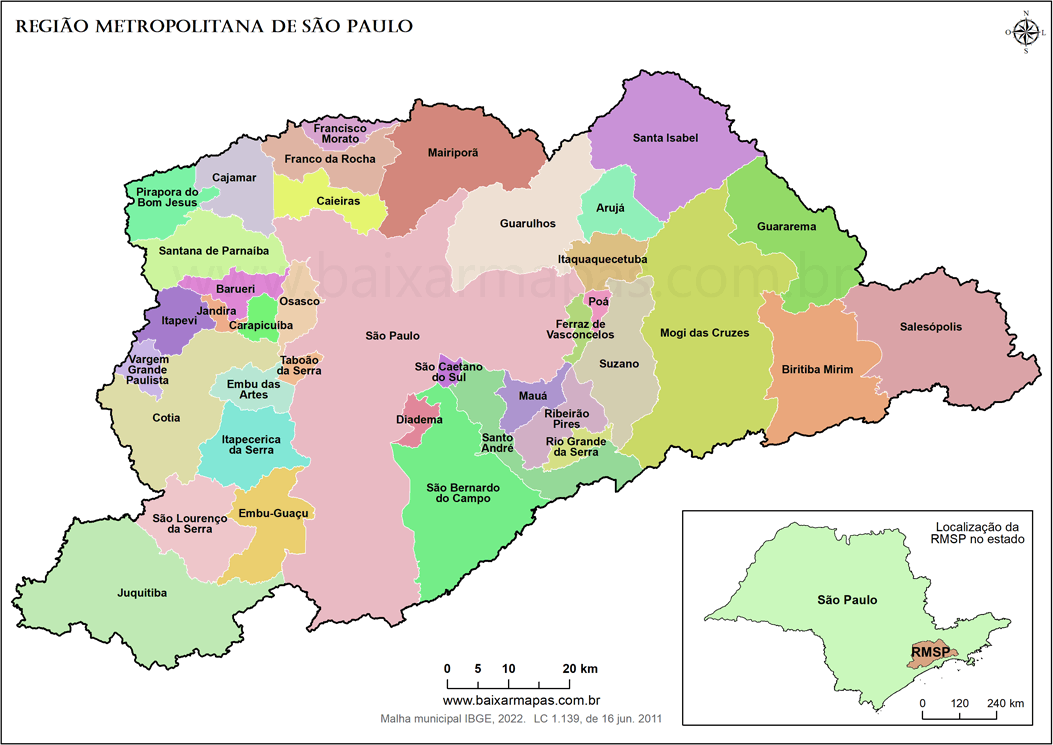
\includegraphics[width=.7\textwidth]{mapa-regiao-metropolitana-sao-paulo-municipios.png}
\caption{Região Metropolitana de São Paulo \cite{baixarmapas2026}}
\label{fig:mapa_rmsp}
\end{figure}

\vspace{1.2cm}

\section{Trabalhos Relacionados}

Com o intuito de mapear o estado da arte e identificar abordagens relacionadas à temática, realizou-se um levantamento bibliográfico que resultou na seleção de três trabalhos diretamente relacionados ao escopo desta pesquisa.

O primeiro estudo selecionado, de \cite{couto2024identificaccao}, investiga padrões comportamentais e espaciais associados ao roubo de celulares no Rio Grande do Sul. O trabalho emprega a técnica de agrupamento não supervisionado K-means integrada a variáveis geográficas e sociodemográficas, buscando correlacionar a incidência do crime às vulnerabilidades socioeconômicas locais. Os resultados evidenciaram que tanto as vítimas quanto os autores dos delitos se concentram majoritariamente em bairros periféricos de Porto Alegre, caracterizados por baixos índices de desenvolvimento humano (IDH) e menor poder aquisitivo.

Paralelamente, \cite{de2025previsao} avaliaram o desempenho comparativo entre Árvores de Decisão e Redes Neurais na predição de roubos de veículos no município do Rio de Janeiro. Embora os resultados tenham demonstrado melhor desempenho preditivo das Redes Neurais no estudo, os autores ressaltam como limitação a menor explicabilidade associada a esse tipo de modelo, aspecto relevante para a tomada de decisões estratégicas em segurança pública.

Por fim, o estudo conduzido por \cite{fernandes2025aplicaccao} investigou os determinantes socioeconômicos e estruturais associados à criminalidade nos municípios do estado de São Paulo. Utilizando o algoritmo XGBoost, o modelo ajustado alcançou um coeficiente de determinação de 98,5\%. A interpretação dos resultados por meio de valores SHAP (\textit{SHapley Additive exPlanations}) foi utilizada para analisar a influência das variáveis consideradas pelo modelo.

A partir do levantamento realizado, observa-se espaço para investigar uma abordagem que combine modelagem preditiva espaço-temporal e representação cartográfica das áreas de maior risco na RMSP. O presente trabalho diferencia-se pelo recorte geográfico da Região Metropolitana de São Paulo, pela delimitação temporal entre 2022 e o primeiro semestre de 2026 e pela análise de diferentes categorias de roubos e furtos, cujo escopo definitivo será estabelecido a partir dos resultados da etapa exploratória. Além disso, serão comparados Random Forest, XGBoost e LightGBM para a modelagem dos dados tabulares.

\vspace{1.2cm}

\section{Metodologia}

Para o desenvolvimento do estudo, foi utilizada a base de dados criminais da Secretaria de Segurança Pública do Estado de São Paulo (SSP-SP)\footnote{\url{https://www.ssp.sp.gov.br/estatistica/consultas} Acesso em: 22/08/2026}, abrangendo o período de 2022 ao primeiro semestre de 2026. As diferentes fontes foram unificadas em um único conjunto de dados e, posteriormente, filtradas para manter os registros de roubos e furtos pertencentes aos municípios da Região Metropolitana de São Paulo. Embora o projeto tenha sido inicialmente direcionado aos roubos, a inclusão dos furtos no escopo da modelagem permanece em avaliação a partir dos resultados obtidos na AED.

Após a consolidação da base, foi realizado o pré-processamento dos dados, incluindo tratamento das informações de município, datas, registros duplicados e coordenadas geográficas. Em seguida, foi conduzida uma Análise Exploratória dos Dados com o objetivo de compreender a distribuição das ocorrências entre cidades, tipos de crime e períodos, além de identificar limitações relacionadas à granularidade espacial e temporal da base.

Para representar a dimensão temporal, as ocorrências foram agrupadas por quinzena. Na dimensão espacial, a análise preliminar mostrou que o uso de latitude e longitude exatas gera unidades excessivamente granulares, com baixa repetição de ocorrências. Por esse motivo, será investigada uma agregação espacial em \textit{grid}, de forma a produzir unidades espaço-temporais mais adequadas ao aprendizado dos modelos.

A modelagem será tratada como um problema de regressão, no qual o objetivo será estimar a quantidade de ocorrências associada a cada unidade espaço-temporal. O escopo definitivo das categorias utilizadas como alvo ainda será definido, considerando os resultados da AED e a possibilidade de modelar roubos e furtos de forma geral ou categorias mais específicas.

Serão comparados os algoritmos Random Forest, XGBoost e LightGBM. O Random Forest será utilizado como modelo de referência, enquanto XGBoost e LightGBM serão empregados como alternativas para comparação de desempenho. O ajuste de hiperparâmetros e a validação deverão preservar a ordem cronológica das observações, evitando que informações futuras sejam utilizadas no treinamento de previsões referentes a períodos anteriores.

Para as etapas de treinamento e validação, será utilizada a série temporal correspondente ao período de 2022 ao primeiro semestre de 2025. O intervalo remanescente, correspondente ao segundo semestre de 2025 e ao primeiro semestre de 2026, será reservado para o teste final. Essa separação temporal busca preservar a cronologia dos dados e avaliar a capacidade de generalização dos modelos em períodos posteriores aos utilizados no treinamento.

O desempenho dos modelos será analisado por meio das métricas MAE, RMSE e $R^2$, adequadas à avaliação das previsões de regressão. Adicionalmente, será utilizado o PAI para avaliar a qualidade espacial das áreas classificadas como \textit{hotspots}. Após a validação, as previsões deverão ser representadas em mapas preditivos de risco para a Região Metropolitana de São Paulo.

\vspace{1.2cm}

\section{Resultados Preliminares}

\subsection{Pré-Processamento da Base de Dados}

Conforme previsto na metodologia, realizou-se a unificação e a padronização das bases de dados. A base original continha 5.348.234 registros referentes a boletins de ocorrência registrados no estado de São Paulo.

A base continha duas colunas relacionadas ao município: \texttt{NOME\_MUNICIPIO\_CIRCUNSCRIÇÃO} e \texttt{NOME\_MUNICIPIO}. A primeira representa o município da circunscrição relacionada à ocorrência, enquanto a segunda corresponde ao município registrado. Aproximadamente 10,3\% dos registros apresentavam valor nulo na primeira coluna. Ao analisar \texttt{NOME\_MUNICIPIO}, verificou-se que não havia valores nulos. Dessa forma, foi criada a coluna \texttt{city}, que utiliza prioritariamente o valor de \texttt{NOME\_MUNICIPIO\_CIRCUNSCRIÇÃO} e, quando este é nulo, utiliza \texttt{NOME\_MUNICIPIO} como valor alternativo.

Antes de derivar mês, dia e ano da ocorrência, foi avaliada a completude das colunas \texttt{DATA\_OCORRENCIA\_BO} e \texttt{DATA\_REGISTRO}. Foram identificados aproximadamente 432 registros sem data de ocorrência do boletim. Devido à baixa representatividade desse volume em relação ao total da base, esses registros foram removidos. Além disso, a coluna \texttt{DATA\_OCORRENCIA\_BO} foi convertida para o tipo \texttt{datetime}, permitindo a extração consistente dos componentes temporais utilizados na análise.

Observou-se que a coluna \texttt{ANO\_BO} representa o ano de registro do boletim de ocorrência e não necessariamente o ano em que o fato ocorreu. Por esse motivo, para garantir consistência na análise temporal, as variáveis de ano, mês e dia foram extraídas a partir da coluna \texttt{DATA\_OCORRENCIA\_BO}.

Embora os arquivos utilizados correspondam ao período entre 2022 e o primeiro semestre de 2026, foram encontrados poucos registros cuja data de ocorrência era anterior a 2022. Esses registros foram considerados inconsistentes com o recorte temporal estabelecido e, portanto, removidos. Não foram identificados registros referentes ao segundo semestre de 2026.

Para definir a granularidade temporal, cada registro foi classificado na primeira ou na segunda quinzena do mês, considerando a primeira quinzena para dias menores ou iguais a 15 e a segunda para os dias posteriores. A partir dessa classificação, foi criada uma chave temporal no formato quinzena-mês-ano, utilizada posteriormente na agregação das ocorrências.

Ao analisar a duplicidade das ocorrências, verificou-se que aproximadamente 0,03\% da base correspondia a registros duplicados. Como esses registros não acrescentavam novas informações à análise, eles foram removidos.

As coordenadas geográficas também foram analisadas, pois são fundamentais para a construção dos mapas preditivos de risco. Foram identificados 285.406 registros em que a latitude, a longitude ou ambas estavam ausentes. Também foram verificadas inconsistências relacionadas à validade das coordenadas, ao sinal esperado e à escala dos valores. Para os registros sem coordenadas válidas, foi adotada a mediana da latitude e da longitude dos demais registros da mesma cidade como estratégia de imputação. Após o tratamento, as coordenadas corrigidas foram utilizadas nas etapas subsequentes.

Por fim, foi produzido um \textit{dataframe} agregado contendo a contagem total e a contagem por tipo de crime para cada combinação de localização e período. Essa estrutura foi utilizada como ponto de partida para a análise da granularidade espaço-temporal e para a preparação da etapa de modelagem.

\vspace{1cm}

\subsection{Análise Exploratória dos Dados (AED)}

Antes de seguir para a modelagem, tornou-se necessário compreender a distribuição da base final, identificando quais cidades concentram mais ocorrências, quais tipos de crime são mais frequentes, como esses registros variam ao longo do tempo e quais limitações da estrutura agregada podem afetar a modelagem espaço-temporal.

\subsubsection{Análise das Ocorrências por Cidade}

\begin{table}[h!]
    \centering
    \begin{tabular}{|l|r|}
        \hline
        \textbf{Cidade} & \textbf{N\textsuperscript{o} de ocorrências} \\
        \hline
        S.PAULO          & 1.860.214 \\
        \hline
        GUARULHOS        & 108.451   \\
        \hline
        S.ANDRE          & 92.778    \\
        \hline
        OSASCO           & 70.236    \\
        \hline
        DIADEMA          & 37.418    \\
        \hline
        MAUA             & 32.376    \\
        \hline
        CARAPICUIBA      & 29.271    \\
        \hline
        MOGI DAS CRUZES  & 28.132    \\
        \hline
        ITAQUAQUECETUBA  & 28.073    \\
        \hline
        SUZANO           & 24.588    \\
        \hline
    \end{tabular}
    \caption{Número de ocorrências por cidade}
    \label{tab:ocorrencias-cidade}
\end{table}

A cidade de São Paulo concentra, sozinha, cerca de 73\% de todas as ocorrências da RMSP presentes na base analisada. Essa concentração é relevante para a modelagem, pois um modelo único para toda a região pode ser fortemente influenciado pelos padrões predominantes da capital, reduzindo a representatividade do comportamento observado nos municípios com menor volume de registros.

\subsubsection{Distribuição por Tipo de Crime}

\begin{table}[h!]
    \centering
    \begin{tabular}{|l|r|}
        \hline
        \textbf{Tipo de crime} & \textbf{\% do total} \\
        \hline
        FURTO - OUTROS       & 56,78\% \\
        \hline
        ROUBO - OUTROS       & 27,65\% \\
        \hline
        FURTO DE VEÍCULO     & 10,84\% \\
        \hline
        ROUBO DE VEÍCULO     & 4,02\%  \\
        \hline
        ROUBO DE CARGA       & 0,66\%  \\
        \hline
        FURTO DE CARGA       & 0,05\%  \\
        \hline
    \end{tabular}
    \caption{Distribuição percentual por tipo de crime}
    \label{tab:crime-percentual}
\end{table}

A categoria \texttt{FURTO - OUTROS} representa mais da metade dos registros da base, seguida por \texttt{ROUBO - OUTROS}. Juntas, essas duas categorias correspondem a mais de 80\% das ocorrências analisadas. Em contrapartida, os registros de furto e roubo de carga apresentam baixa frequência relativa. Essa distribuição evidencia tanto o desbalanceamento entre as categorias quanto a dificuldade de trabalhar exclusivamente com tipologias mais específicas.

\subsubsection{Distribuição Temporal por Ano}

\begin{table}[h!]
    \centering
    \begin{tabular}{|l|l|}
        \hline
        \textbf{Ano} & \textbf{N\textsuperscript{o} de ocorrências} \\
        \hline
        2022 & 593.039 \\
        \hline
        2023 & 595.336 \\
        \hline
        2024 & 558.717 \\
        \hline
        2025 & 531.594 \\
        \hline
        2026 & 240.435 (ano parcial) \\
        \hline
    \end{tabular}
    \caption{Número de ocorrências por ano}
    \label{tab:ocorrencias-ano}
\end{table}

O volume de ocorrências permanece relativamente estável entre 2022 e 2025, embora seja observada uma tendência de redução a partir de 2023. O número referente a 2026 é inferior aos demais porque a base utilizada contém apenas os registros do primeiro semestre desse ano. A análise mensal por ano também indica a repetição de um padrão semelhante ao longo dos períodos observados, sem diferenças relevantes além da tendência geral de redução já identificada.

\vspace{1cm}

\subsection{Métricas}

Foram selecionadas quatro métricas para avaliar o desempenho dos modelos e permitir a comparação entre Random Forest, XGBoost e LightGBM. MAE, RMSE e $R^2$ serão utilizadas para avaliar as previsões de regressão, enquanto o PAI será empregado para avaliar a qualidade espacial das regiões classificadas como \textit{hotspots}.

\noindent
\textbf{MAE (\textit{Mean Absolute Error} -- Erro Absoluto Médio):} mede, em média, o quanto as previsões do modelo diferem dos valores observados, considerando apenas a magnitude do erro, independentemente de a previsão ser superior ou inferior ao valor real. Uma de suas principais vantagens é a interpretação direta, pois o resultado permanece na mesma unidade da variável prevista. Quanto menor o MAE, menor é o erro absoluto médio do modelo.

\[
MAE = \frac{1}{n}\sum_{i=1}^{n}|y_i-\hat{y}_i|
\]

Em que:
\begin{itemize}
    \item $n$ é o número total de observações;
    \item $y_i$ é o valor real;
    \item $\hat{y}_i$ é o valor previsto pelo modelo.
\end{itemize}

Por exemplo, se $MAE = 2{,}3$, isso significa que, em média, a previsão do modelo difere da quantidade real em aproximadamente 2,3 ocorrências por unidade espaço-temporal, definida no projeto pela combinação entre região espacial e quinzena.

\vspace{1.2cm}
\noindent
\textbf{RMSE (\textit{Root Mean Squared Error} -- Raiz do Erro Quadrático Médio):} também mede a diferença entre os valores previstos e observados, porém atribui maior peso aos erros de maior magnitude porque as diferenças são elevadas ao quadrado antes do cálculo da média. Essa característica permite identificar modelos que, embora apresentem erros médios aceitáveis, podem cometer discrepâncias elevadas em determinadas observações.

\[
RMSE =
\sqrt{
\frac{1}{n}
\sum_{i=1}^{n}
(y_i-\hat{y}_i)^2
}
\]

Por exemplo, um resultado de $MAE = 2{,}1$ e $RMSE = 7{,}8$ pode indicar que grande parte das previsões apresenta erro relativamente baixo, mas existem algumas observações com erros consideravelmente maiores.

\vspace{1.2cm}
\noindent
\textbf{$R^2$ (\textit{Coefficient of Determination} -- Coeficiente de Determinação):} mede quanto da variabilidade presente nos valores observados é representada pelas previsões do modelo. Enquanto MAE e RMSE medem diretamente a magnitude dos erros, o $R^2$ compara o desempenho do modelo com uma referência baseada na média dos valores observados.

\[
R^2 =
1 -
\frac{
\sum_{i=1}^{n}(y_i-\hat{y}_i)^2
}{
\sum_{i=1}^{n}(y_i-\bar{y})^2
}
\]

Em que:
\begin{itemize}
    \item $y_i$ é o valor real;
    \item $\hat{y}_i$ é o valor previsto;
    \item $\bar{y}$ é a média dos valores reais.
\end{itemize}

Quando $R^2 = 1$, há ajuste perfeito entre os valores previstos e observados. Quando $R^2 = 0$, o modelo não apresenta vantagem, segundo essa métrica, em relação a uma previsão constante baseada na média. Valores de $R^2 < 0$ indicam desempenho inferior a essa referência. Por exemplo, $R^2 = 0{,}72$ indica que aproximadamente 72\% da variabilidade observada é representada pelo modelo no conjunto avaliado.

\vspace{1.2cm}
\noindent
\textbf{PAI (\textit{Prediction Accuracy Index} -- Índice de Acurácia da Predição):} será utilizado para avaliar a qualidade espacial das áreas identificadas como \textit{hotspots}. Diferentemente das métricas anteriores, seu objetivo não é avaliar diretamente a diferença entre a quantidade prevista e a quantidade observada, mas verificar se as áreas indicadas pelo modelo como de maior risco concentram uma parcela elevada das ocorrências observadas posteriormente. Para aplicar essa métrica, será necessário definir um critério para delimitar as áreas classificadas como \textit{hotspots}.

Uma forma de representá-lo é:

\[
PAI =
\frac{\text{Hit Rate}}{\text{proporção da área classificada como hotspot}}
\]

O \textit{Hit Rate} representa a proporção das ocorrências observadas que se encontram dentro das áreas consideradas \textit{hotspots}:

\[
\text{Hit Rate} =
\frac{\text{ocorrências nos hotspots}}{\text{total de ocorrências}}
\]

Quanto maior o PAI, maior é a concentração relativa das ocorrências nas áreas classificadas como de maior risco.

\vspace{1.2cm}

\section{Discussão e Conclusão}

Ao longo da Análise Exploratória dos Dados (AED), identificamos que o alvo inicialmente definido para o projeto, os roubos, apresentava um volume de ocorrências menor do que o esperado. Além disso, observamos uma dificuldade relevante na identificação do tipo específico de roubo associado a determinadas ocorrências da base. Diante desse cenário, verificamos que a inclusão dos furtos poderia ampliar significativamente a quantidade de dados disponível para o treinamento do modelo. Por esse motivo, ainda será avaliada a possibilidade de ampliar o escopo da pesquisa, considerando tanto roubos quanto furtos, seja em categorias específicas relacionadas a pedestres, seja de forma mais geral.

Conceitualmente, a principal diferença entre furto e roubo está na presença de violência ou grave ameaça contra a vítima. No furto, ocorre a subtração de um bem alheio sem o uso de violência ou grave ameaça, como no caso de um celular retirado de uma mochila sem que a vítima perceba. Já no roubo, a subtração ocorre mediante violência ou grave ameaça, como em uma situação na qual a vítima é abordada com o uso de força física ou de uma arma.

Outro aspecto relevante identificado durante a análise é a elevada concentração das ocorrências na cidade de São Paulo, que representa mais de 70\% dos registros da base analisada. Essa concentração deve ser considerada na etapa de modelagem, pois pode fazer com que os padrões predominantes da capital exerçam maior influência sobre o comportamento aprendido pelo modelo em relação aos demais municípios.

O principal desafio identificado para a continuidade do projeto é a elevada granularidade espacial da base agregada, que pode dificultar o aprendizado dos modelos. O \textit{dataframe} final foi inicialmente agrupado por latitude e longitude exatas e por quinzena. Como coordenadas geográficas com várias casas decimais raramente se repetem entre diferentes registros, grande parte das unidades espaço-temporais aparece apenas uma vez, reduzindo a quantidade de repetições a partir das quais o modelo poderia aprender padrões locais de maior ou menor incidência. Para evidenciar esse problema, foi comparada a granularidade espacial original com uma agregação em \textit{grid}, obtida por meio do arredondamento da latitude e da longitude para duas casas decimais, correspondendo aproximadamente a células de 1,1 km.

Comparando as duas granularidades espaciais na base final analisada, correspondente ao período entre 2022 e o primeiro semestre de 2026 e contendo aproximadamente 1,79 milhão de unidades agregadas na configuração original, obtiveram-se os resultados apresentados na Tabela~\ref{tab:granularidade}.

\begin{table}[H]
\centering
\caption{Comparação entre diferentes granularidades espaciais}
\label{tab:granularidade}

\renewcommand{\arraystretch}{1.5}

\begin{tabularx}{\textwidth}{
    |>{\raggedright\arraybackslash}X
    |>{\centering\arraybackslash}m{2cm}
    |>{\centering\arraybackslash}m{3cm}
    |>{\centering\arraybackslash}m{1.7cm}
    |>{\centering\arraybackslash}m{3.1cm}|
}
\hline

\textbf{Granularidade} &
\textbf{N\textsuperscript{o} de células} &
\textbf{Média de ocorrências/célula} &
\textbf{Mediana} &
\textbf{\% de células com apenas 1 ocorrência} \\

\hline

Lat./Long. exatas + quinzena (\textit{dataframe} original) &
1.789.422 &
1,41 &
1 &
\textbf{90,81\%} \\

\hline

Grid $\sim$1,1 km (2 casas decimais) + quinzena &
201.695 &
12,49 &
6 &
\textbf{20,20\%} \\

\hline
\end{tabularx}

\end{table}

Os resultados reforçam a limitação da agregação original. Nessa configuração, 90,81\% das células apresentam apenas uma ocorrência, o que reduz a repetição de observações em uma mesma unidade espacial. Com a agregação aproximada em \textit{grid} de 1,1 km, esse percentual cai para 20,20\%, enquanto a mediana passa de 1 para 6 ocorrências por célula. Esses resultados indicam que a definição da unidade espacial será uma etapa determinante antes do treinamento dos modelos.

Assim, as próximas etapas deverão concentrar-se na definição do escopo final das categorias de crime e da granularidade espacial utilizada na modelagem. A partir dessas decisões, será possível estruturar as unidades espaço-temporais, treinar e comparar Random Forest, XGBoost e LightGBM e, posteriormente, avaliar as previsões tanto pelas métricas de regressão quanto pela capacidade de identificar espacialmente áreas de maior concentração de ocorrências.

\vspace{1.2cm}

\bibliographystyle{plain}
\bibliography{referencias}

\end{document}





Quantidade máxima de páginas por seção:
Título e resumo 1 página
Introdução  2 páginas
Método 2 páginas
Trabalhos correlatos 3 páginas
Resultados preliminares (análise exploratória dos dados) 3 páginas
Discussão e conclusão 1 página